% This must be in the first 5 lines to tell arXiv to use pdfLaTeX, which is strongly recommended.
\pdfoutput=1
% In particular, the hyperref package requires pdfLaTeX in order to break URLs across lines.

\documentclass[11pt]{article}

% Remove the "review" option to generate the final version.
\usepackage{./figs-misc/acl2023}
\pagestyle{plain}

% Standard package includes
\usepackage{times}
\usepackage{latexsym}

% For proper rendering and hyphenation of words containing Latin characters (including in bib files)
\usepackage[T1]{fontenc}
% For Vietnamese characters
% \usepackage[T5]{fontenc}
% See https://www.latex-project.org/help/documentation/encguide.pdf for other character sets

% This assumes your files are encoded as UTF8
\usepackage[utf8]{inputenc}

% This is not strictly necessary, and may be commented out.
% However, it will improve the layout of the manuscript,
% and will typically save some space.
\usepackage{microtype}

% This is also not strictly necessary, and may be commented out.
% However, it will improve the aesthetics of text in
% the typewriter font.
\usepackage{inconsolata}

\usepackage{linguex}
\usepackage{csquotes}
\usepackage{caption}
\usepackage{graphicx}

% If the title and author information does not fit in the area allocated, uncomment the following
%
%\setlength\titlebox{<dim>}
%
% and set <dim> to something 5cm or larger.

\title{Dialectic Bias in Toxicity Detection of Google's Perspective API
\bigbreak A study with five parallel corpora}

% Author information can be set in various styles:
% For several authors from the same institution:
% \author{Author 1 \and ... \and Author n \\
%         Address line \\ ... \\ Address line}
% if the names do not fit well on one line use
%         Author 1 \\ {\bf Author 2} \\ ... \\ {\bf Author n} \\
% For authors from different institutions:
% \author{Author 1 \\ Address line \\  ... \\ Address line
%         \And  ... \And
%         Author n \\ Address line \\ ... \\ Address line}
% To start a seperate ``row'' of authors use \AND, as in
% \author{Author 1 \\ Address line \\  ... \\ Address line
%         \AND
%         Author 2 \\ Address line \\ ... \\ Address line \And
%         Author 3 \\ Address line \\ ... \\ Address line}

\author{Hanxin Xia $\vert$ 3417418\\
  \href{mailto://hanxin.xia@uni-duesseldorf.de}{hanxin.xia@uni-duesseldorf.de}}

\begin{document}
\maketitle

\begin{abstract}
Hate Speech detection has been a heated topic in NLP/NLU since the spread of social media. Despite the existence of various automatic toxicity scoring models, their biases against language varieties that align with minority identities have been discussed by researchers \citep{sap-etal-2019-risk}. In this work, we focus on Google's Perspective API and analyze its toxicity scores on four synthetic corpora with different dialect features compared to an original master corpus. We discovered that Perspective API scored all four parallel corpora significantly differently from the master corpus, which further confirms the existence of the biases. Moreover, we discovered the capping phenomenon with the toxicity scores of the gold toxic sentences: Gold non-toxic sentences are more liketly to suffer from toxicity score increase, when converted to a dialect, compared to gold toxic sentences.
\end{abstract}


\section{Introduction}

With the increasing popularity of social media and the daily widening user bases, the moderation of the contents on online communication platforms have been a crucial part of maintaining the friendliness for the users and building healthy communities. In pursuit of this objective, the platforms have implemented various means including reactive methods such as community guidelines, user report and post-removal of harmful contents and proactive methods either with sensitive words and language pattern rules \citep{gitari-2015-lexicon} or machine learning algorithms for automated hate speech detection \citep{alrehili-2019-survey}.

However current detoxifying approaches are proven to be not perfect. While the reactive methods are commonly subject to deficiency and passivity, the automatic proactive methods often discriminate against minority aligned language varieties other than Standard American English (SAE) \citep{sap-etal-2019-risk, zhou-etal-2021-challenges}.

This research aims to test the performance of Google’s Perspective API on five parallel corpora. Despite being a continuously improving model on toxicity scoring \citep{google-perspective}, the bias against non-standard English is still present in the results. The model scored (state: March 2024) texts from the four English dialects: African American Vernacular English (AAVE), Nigerian and Indian dialects and Singaporean English (Singlish). significantly differently than the original texts of standard English. Thus, we posit that there is a continued need for optimization in the hate speech detection of online contents for better mitigating biases that may infringe upon the online representation of individuals from marginalized communities.


\section{Background}

The process of detoxification and hate speech detection is aimed to create healthy and welcoming online communities. Yet the biases in these processes are leading to not only unfair penalties for minority individuals \citep{davidson-etal-2019-racial} but also potential complete exclusion of their voices in online spaces \citep{blodgett-2017-racial} simply because of the usage of non-standard language.

The underlying reasons behind such biases can be traced back to multiple factors. As \citet{xia-etal-2020-demoting} and \citet{sap-etal-2022-annotators} point out, first-hand annotators are inclined to classify non-abusive AAE texts as toxic, which may lead to bias already at the corpus creation stage. Secondly, surface markers on the language such as mention of specific identity terms and usage of certain uncommon patterns are also prone to cause the so-called \enquote{key word bias} in models \citep{resende-2024-comprehensive, schafer-2023-bias}. The lack of data of English language varieties in the training data may lead to their incapability to capture the real intentions and deep meanings of such speeches. Last but not the least, suboptimal performances of hate speech detection models can also be attributed to the ignorance of linguistic subtleties engrained in contextual factors such as speaker identity, environment and even special spelling \citep{davidson-etal-2019-racial}.

Several methodologies have been proposed to mitigate these biases. \citet{schafer-2023-bias} experimented with transformer based multi-class prediction in order to establish a more comprehensive viewpoint for hate speech detection with less success. Moreover, the approach of masking out identity terms exhibits obvious drawbacks despites its merits. By raising subjectivity level when identity terms occur, \citep{zhao-2022-subjectivity} were able to efficiently neutralize their model’s bias against minority aligned texts. Similar effects can be achieved by including confident dialect prediction \citep{ball-2021-differential}. By implementing adversarial learning during the model learning process, \citet{xia-etal-2020-demoting} and \citep{okpala-2022-aaebert} were both able to reduce baseline model’s false positive rate facing African American English like texts.


\section{Data}

This section provides an overview on the dataset used in this research. The data augmentation and synthesizing technique will be explained. The choice of the synthetic approach will also be substantiated.

\subsection{HateXplain} \label{hatexplain-data}

The data the research is based on stems from the publicly available HateXplain\footnote{\url{https://github.com/hate-alert/HateXplain}} dataset. HateXplain is designed for interpretation of hate speech detection results based on certain text features. It includes 20,148 instances from Twitter and Gab posts collected around the year 2020. Besides the class labeling (\textit{hate}, \textit{offensive} or \textit{normal}), targeted groups and rationales (text chunk that directly contributes to the decision) are also included in the annotation scheme. Each post is annotated by three Amazon Mechanical Turk (MTurk) workers. 919 instances, where all three annotators decide for a different class, are excluded from the final compilation, which ensures the credibility of the annotation results \citep{mathew-2021-hatexplain}.

Since the original class label is tri-partie and the dichotomy of toxicity is interested in the research, we combine \textit{hate} and \textit{offensive} together as toxic, and reinterpret \textit{normal} as non-toxic. Based on majority voting among the three annotators, we are able to retrieve 12,276 toxic and 7,771 non-toxic posts.

The HateXplain dataset with the newly interpreted labels will be referred to as the \textbf{original} or \textbf{master dataset} in the following texts.

\subsection{Synthetic datasets}

Acknowledging the restricted capabilities of current NLP systems on different English language varieties, the Multi-VALUE\footnote{\url{https://github.com/SALT-NLP/multi-value/tree/main}} package \citep{ziems-2023-multi} provides a complete framework for rule-based English dialect transformation and evaluation. By applying syntactic and morphological transformation rules based on 189 unique features, Multi-VALUE is able to convert SAE to 50 English dialects.

In this experiment, we choose four representative dialects: African American Vernacular English (\textbf{AAVE}), Nigerian English (\textbf{NigerianD}), Indian English (\textbf{IndianD}) and Colloquial Singapore English (\textbf{Singlish}). The selection includes English dominant communities spanning across three major continents with different historic relations with the English language, which provides good representativeness on the general tendency comparing standard English and dialects.

To measure the distinction of the dialect coded texts, the rules applied on each instance are saved as references. Among the 100 most used rules for each dialect conversion, only 13 of them overlap. This indicates the transformation features are relatively specific to each dialect and inter corpora differences among the synthetic data is high. Examples for most used rules for transformation to each dialect can be found in Appendix \ref{rules}.

In the end, all 20,148 texts from the master dataset were successfully converted to dialect.

\subsection{Data choice}

Most of the research focused on bias in toxicity detection so far are based on two separate sets of text data \citep{sap-etal-2019-risk, davidson-etal-2019-racial, ball-2021-differential, zhou-etal-2021-challenges}. The data could be sourced from the same domain (i.e. the same social media platform) and split into two subsets. One for standard English and one for texts with certain dialect features. Such an approach ensures the authenticity of the data, since they are real interactions of users online. However, there is no real correlation between the texts in those two subsets. At the same time, manual splitting the data requires extra labor. The subjectivity of the annotators may also lead to inaccuracy of categorization of different dialects. Moreover, scarcity has always been an issue while dealing with minority aligned language usage \citep{dash-2019-scarcity}. Even on social media, where dialect styled writings are more frequent, the data with such features are still scarce and costly to collect \citep{jorgensen-2015-challenges}. These issues are the underlying reasons for the inability to scale in the research focused on dialects and low resource languages.

The advantage of Multi-VALUE in this respect is that we can augment a large number of text data with features specific to certain dialects under the investigation of a study. Using data augmentation to combat scarcity issues is a common approach \citep{bird-2020-augmentation}. While partly sacrificing the authenticity of the data, Multi-VALUE shows strong capability of preserving meaning and ensuring syntactic integrity and naturalness \citep{ziems-2022-value, ziems-2023-multi}.

Because the augmented data is 1:1 parallel to that in the master dataset, we are able to investigate the behaviors of one instance with or without dialect features individually. Other than that, by applying multiple conversions, larger scale studies on multiple dialects are also possible, without massive investment in time and energy. Finally, while examining the toxicity score changes after conversion, by backtracking the transformation rules that were used for the conversion, it is also possible to identify the dialect specific features that are responsible for the increase or decrease in text toxicity. This would not be possible if only collected data are used, unless every feature in the dialect data is readily available.

\section{Methodology}

Perspective API is a multilingual machine learning model for identifying abusive comments developed by Google \citep{jigsaw-2017-perspective}. It has been in constant development since its introduction. The data are sourced from online forums and all manually annotated. The quality of the annotations is ensured by 3-10 annotators per sentence. Being trained on such in-house compiled datasets, Perspective API provides a useful metric to detect hate speech texts from HateXplain dataset without causing data contamination.

All sentences in the five parallel corpora with differently styled English were passed directly to Google’s Perspective API for toxicity scoring using Google Colaboratory platform (access date: March 2024). Because of the 1 request per second rate limit of Perspective, we defined a 0.8 second wait time after successfully retrieving the score of the current sentence. The data were split into 4 batches with 5000 each to address the access time restriction of Google Colab.

\section{Results}

As a multilingual model, Perspective API also suffers from the error of misclassifying non-standard English as non-English discussed by \citet{davidson-etal-2019-racial}. Hence the indexes of the errors caused by false language identification are saved for results filtering. The error indexes in all batches of the five corpora are then unionized and their corresponding instances are removed in parallel. In the end, we were able to retrieve 20,047 valid results from the Perspective API.

The continuous percentile ratings of the toxicity of each text are reinterpreted based on the 50\% threshold as categorical classes. To summarize, there were 12,089 instances from the original data, 11,819 from AAVE, 12,057 from Nigerian dialect, 11,684 from Indian dialect and 12,053 from Singlish labeled as toxic by Perspective API. All numbers are in line with the 12,276 toxic counts rated by \citet{mathew-2021-hatexplain}.

\begin{figure*}[t]
  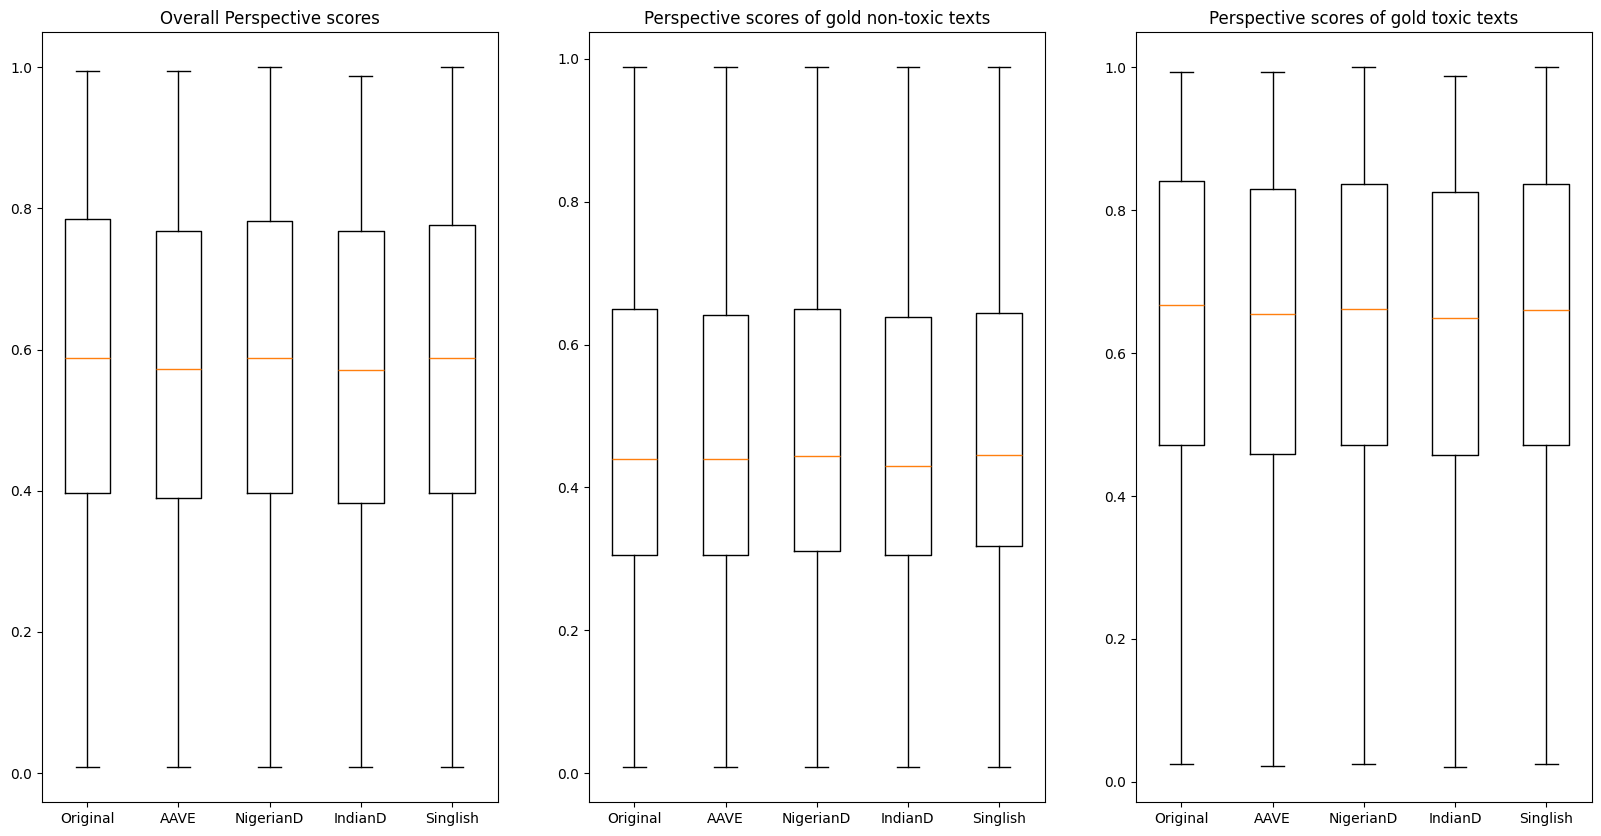
\includegraphics[width=1.0\linewidth]{figs-misc/all-scores.png}
  \caption{Toxicity scores of texts in five parallel corpora based on HateXplain by Perspective API. 1 = toxic; 0 = non-toxic. Overall score tendencies of all texts are shown in the first plot. The 2nd and the 3rd graph shows the inter-corpora score differences in gold non-toxic and toxic subsets.}
  \label{all-scores}
\end{figure*}

\subsection{Reliability of Perspective API's scores}

Since Perspective API’s scores for different corpora are being compared here, the gold labels in HateXplain are not directly used in the data analysis. However, it provides a standard for reference for evaluating the validity of Perspective’s scores on the master corpus.

For this purpose we conducted a Chi-square test on the redacted gold toxic labels from the master data as explained in Chapter \ref{hatexplain-data} and Perspective’s classification results for the original texts without conversion. The test returned a \textit{p}-value of 0.0, indicating statistical significance well below the common threshold of 0.05, alongside a large Chi-square statistic of 1799.35. Both metrics reveal a high degree of association between gold labels and the class assignments by Perspective API.

From the test results and the similar proportion of toxic labels between the gold and prediction, we therefore conclude the Perspective API's toxicity scores on the original texts are fairly similar to the gold labels. I.e., Perspective API can be considered reliable for the research purpose.

\subsection{Inter-corpora comparison of toxicity score}

It is worth mentioning that this research is interested in one same hate speech detection model’s performance differences facing SAE and dialect coded parallel texts. Hence, Perspective API’s scores of the master corpus are considered as the baseline to be compared to other four corpora. The score results are shown in Figure \ref{all-scores}.

As the first plot suggests, the overall toxicity scores of four synthetic datasets are similar to those of the original dataset. By simply checking the score means of the five groups, it seems to indicate Perspective API has overcome the dialect bias (original: 58.09\%; AAVE: 57.16\%; NigerianD: 58.00\%; IndianD: 56.83\%; Singlish: 57.96\%)

However, given the fact that the observations in each corpus are highly correlated with 1:1 parallelism, simply comparing the overall tendency would not bring the most accurate interpretation of the results. Hence, we chose to further apply a paired t-test on each original vs. dialect combination, which allows us to better determine if there is a statistically significant difference between the means of our two datasets by accounting for the inherent pairing of the observations. The test statistics are shown in Tabel \ref{paired-overall}.

The \textit{p}-values from all paired t-test results are far below the common threshold 0.05. Based on this statistic we are able to reject the null hypothesis and reach the conclusion that Perspective API scores texts with dialect features significantly differently than the original texts without.

\begin{table}[t]
\centering
\begin{tabular}{lr}
\hline
\textbf{original vs.} & \textbf{\textit{p}-value}        \\ \hline
\textbf{AAVE}         & 1.6911696758094217e-206 \\
\textbf{NigerianD}    & 0.00025315431841845546  \\
\textbf{IndianD}      & 5.986704613429082e-281  \\
\textbf{Singlish}     & 0.0004036007665723802   \\ \hline
\end{tabular}
\caption{Paired t-test results of all combinations.}
\label{paired-overall}
\end{table}

\begin{figure*}[t]
  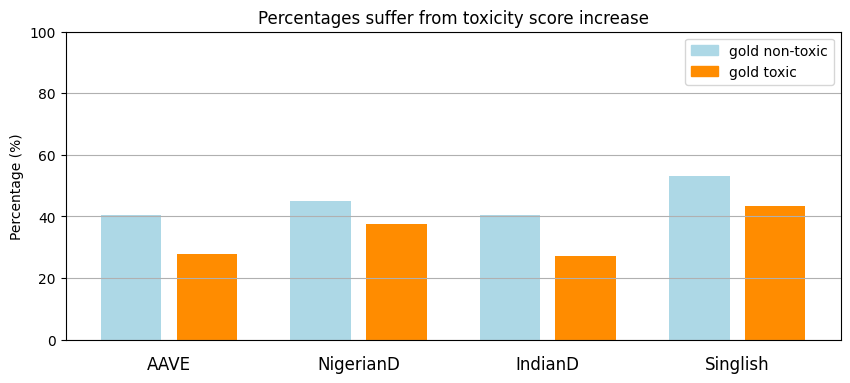
\includegraphics[width=1.0\linewidth]{figs-misc/score-increase-percentages.png}
  \caption{Percentages of instances form different dialect subsets that experience toxicity score increase compared to original unconverted texts. Each dialect set is split based on gold label in order to illustrate whether gold toxic or non-toxic texts suffer more from socre increase.}
  \label{inc-percentages}
\end{figure*}

By splitting the results based on gold toxicity classes, the phenomenon still seems to persist. The right two plots in Figure \ref{all-scores} suggest, the score means of the dialect texts inside the gold toxic or non-toxic class are similar to those of the instances in master corpus of the corresponding class, so are the overall distributions. However, upon further inspection of the paired t-tests results, we discovered that inside the non-toxic class, all original vs. dialect pairs are consistently proven to be significantly different (original vs. AAVE: \textit{p}-value = 1.20946528341701e-21; original vs. NigerianD: \textit{p}-value = 1.0785895427150844e-06; original vs. IndianD: \textit{p}-value = 6.692747637347256e-37; original vs. Singlish: \textit{p}-value = 4.4973972765103815e-09).

The same holds true for gold toxic class (original vs. AAVE: \textit{p}-value = 1.3663633663741608e-218; original vs. NigerianD: \textit{p}-value = 2.696504369252737e-20; original vs. IndianD: \textit{p}-value = 1.9198610161306423e-285; original vs. Singlish: \textit{p}-value = 1.6843712377622434e-23).

Therefore, we conclude that despite similar overall score means of the master and the rest four parallel corpora, Perspective API’s toxicity scores exhibit strong inter-corporal differences when considering individual instances.

\subsection{Toxicity score cappping}

A hypothesis mentioned earlier is that there could be an asymmetry on how automatic toxicity scoring models react to different types of parallel texts based on their gold labels. Namely, when facing gold toxic texts, Perspective API would not score dialect aligned texts higher than their SAE counterparts, as the scores of the original texts are already high. But when it comes to the texts that are originally not toxic, the dialects are more likely to be scored higher due to certain syntactic features and surface markers.


Upon inspecting the scores, we find that among the 7,771 gold non-toxic texts with valid scores from the Perspective API, 3,142 (40.43\%) of them suffer from an increase in toxicity when converted to AAVE. When converted to Nigerian, Indian and Singaporean English, 3,507 (45,13\%), 3,136 (40.36\%) and 4,131 (53.16\%) of these texts respectively exhibit a similar increase in toxicity. Among the 12,276 gold toxic texts, the ratio experiencing toxicity increase after dialect conversion is significantly smaller, with Singlish suffering from most (5,311, 43.26\%), followed by Nigerian dialect (4,591, 37.4\%) and AAVE (3,418, 27.84\%). And mere 3,348 (27.27\%) Indian English texts with gold toxic labels underwent a score increase. The percentages of gold non-toxic texts that are scored more toxic in dialect are consistently higher than that of the gold toxic texts (see in Figure \ref{inc-percentages}).

The same can be observed on the data points on the second and third quartiles (Q2 and Q3) of the dataset. Since the distribution of the toxicity scores ranges from almost 0 to almost full 1.0 (see in Figure \ref{all-scores}), focusing on Q2 and Q3 provides a more centralized perspective, effectively minimizing the influence of outliers and offering a clearer insight into the typical characteristics of the data. Figure \ref{q2-q3} shows the toxicity changes of instances in master corpus and parallel instances in dialect corpora. In each dialect subplot, the left plot shows the subset of gold non-toxic whereas the right shows the gold toxic instances. The individual scores increasing and decreasing are indicated using orange and blue lines respectively. As the orange line density indicates, in the middle quartiles as well, a larger proportion of the gold non-toxic set displays a rise in toxicity scores compared to gold toxic subsets.

\begin{figure*}[t]
  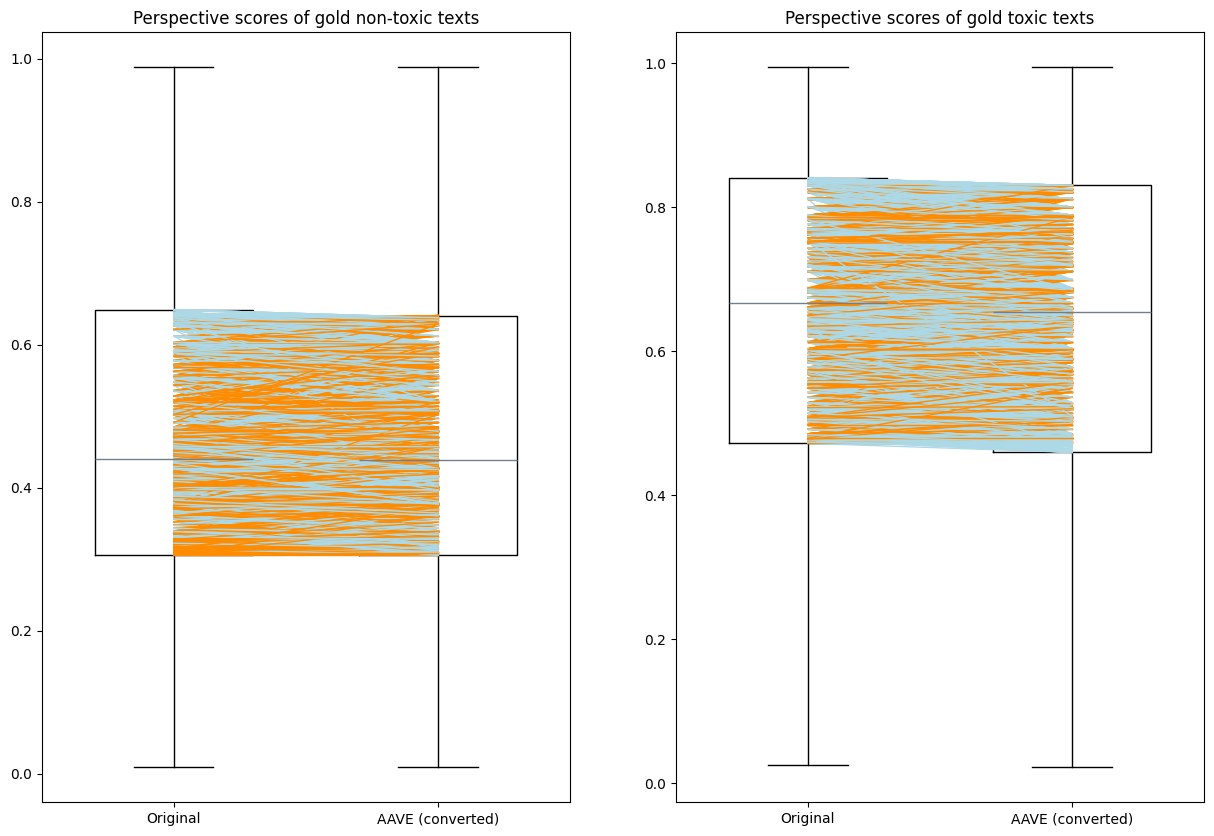
\includegraphics[width=0.48\linewidth]{figs-misc/AAVE-changes.png}\hfill
  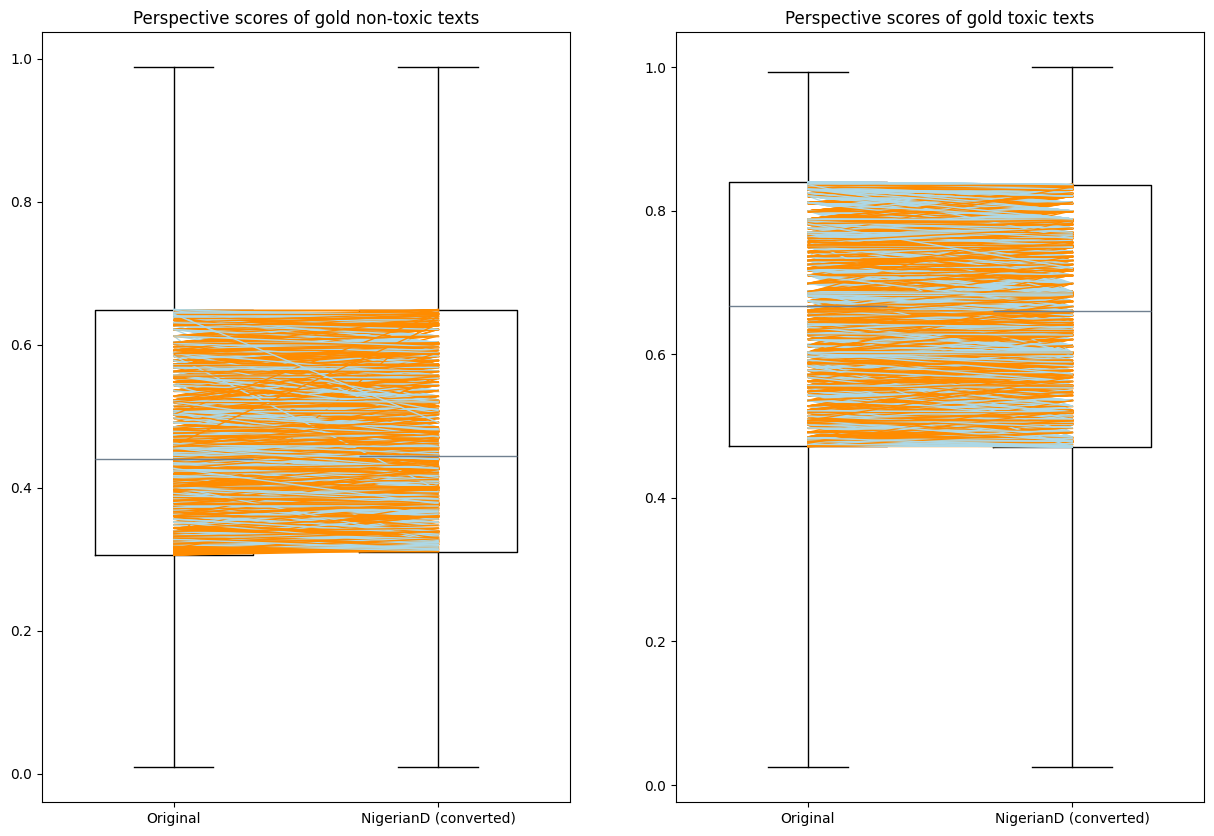
\includegraphics[width=0.48\linewidth]{figs-misc/NigerianD-changes.png}\bigbreak
  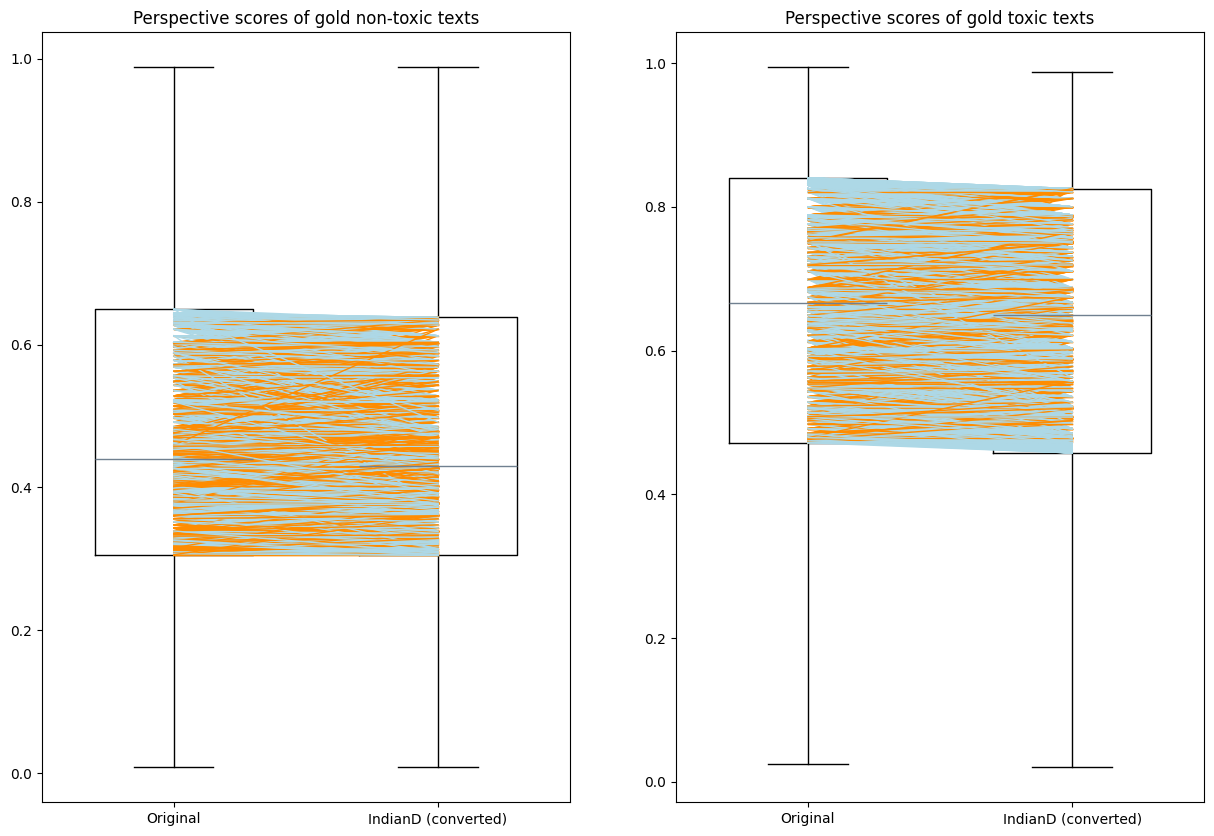
\includegraphics[width=0.48\linewidth]{figs-misc/IndianD-changes.png}\hfill
  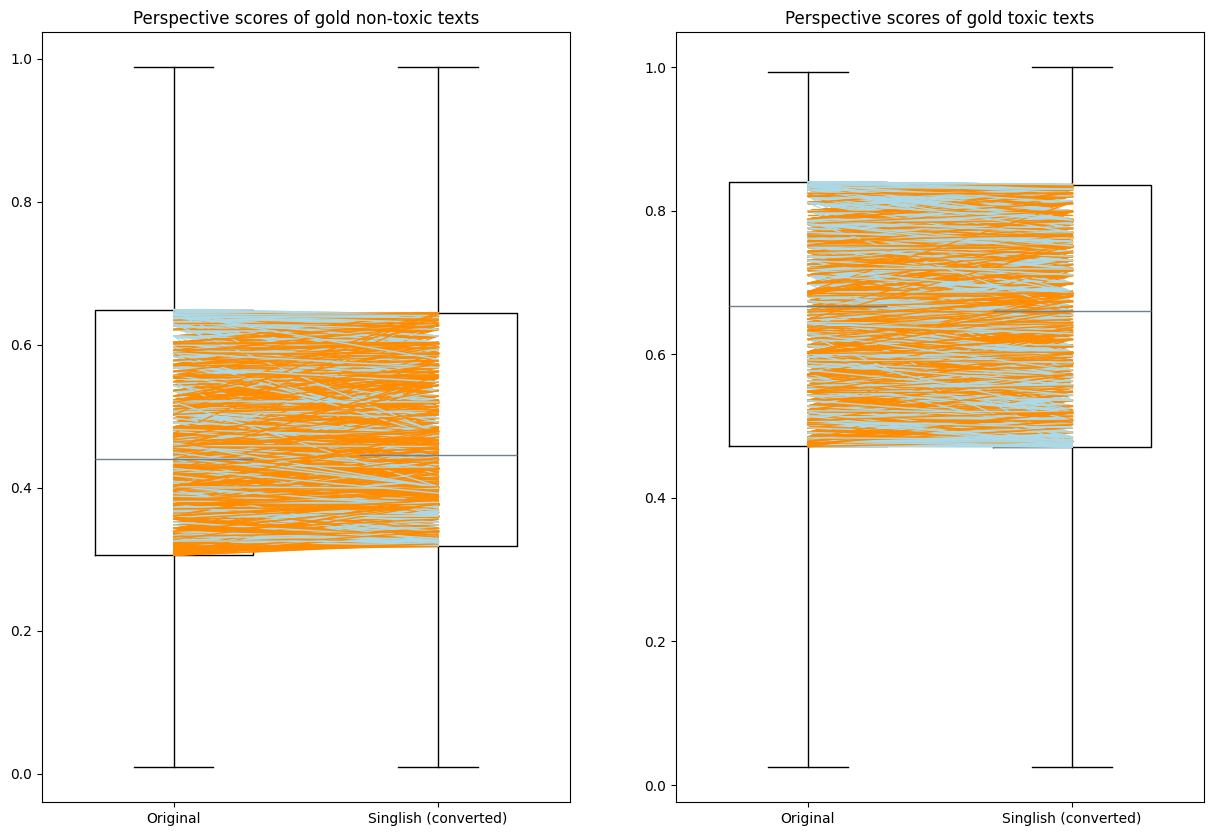
\includegraphics[width=0.48\linewidth]{figs-misc/Singlish-changes.png}
  \caption{Changes in toxicity score of each instance betwenn the original and synthetic dialect set. Each original vs. dialect pair is split into two parts based on gold non-toxic and toxic label. Orange line indicates toxicity increasing on one instance when it is converted to dialect. Blue line indicates decreasing.}
  \label{q2-q3}
\end{figure*}

\newpage

As for the disparity of increase in degree, we found across all four dialect subsets, the toxicity scores of gold non-toxic sentences generally increase more than the toxic sentences. The toxicity scores of the non-toxic instances increased 2.5\% on average when converted to AAVE, as opposed to 2.2\% for gold toxic sentences. The asymmetry can also be found in all other three dialects (NigerianD: 2.6\% vs. 2.1\%; IndianD: 2.9\% vs. 2.5\%; Singlsih: 3.6\% vs. 2.9\%).



































\newpage





\section{Conclusion}

\section{Future Studies}



% Entries for the entire Anthology, followed by custom entries
\bibliography{references}
\bibliographystyle{./figs-misc/acl_natbib}


\appendix

\section{Code access}

Source code and detailed instructions for conducting analyses are publicly accessible under: \href{https://github.com/xuanxuanx-98/ToxBias-ParallelCorpora}{https://github.com/xuanxuanx-98/ToxBias-ParallelCorpora}.

\section{Rule frequency for dialect conversion} \label{rules}

\begin{center}
\begin{tabular}{lr}
\hline
\textbf{rule name}                     & \textbf{frequency} \\ \hline
yall                                   & 4379               \\
demonstrative\_for\_definite\_articles & 4197               \\
mass\_noun\_plurals                    & 4112               \\
regularized\_plurals                   & 4083               \\
uninflect                              & 3595               \\
zero\_plural                           & 2540               \\
null\_relcl                            & 2401               \\
double\_modals                         & 2303               \\
drop\_copula\_be\_NP                   & 2294               \\
progressives                           & 2277               \\ \hline
\end{tabular}
\captionof{table}{Top 10 rules used for converting to African American Vernacular English.}
\end{center}

\begin{center}
\begin{tabular}{lr}
\hline
\textbf{rule name}         & \textbf{frequency} \\ \hline
null\_prepositions         & 8651               \\
mass\_noun\_plurals        & 8476               \\
remove\_det\_definite      & 7326               \\
progressives               & 6964               \\
drop\_inf\_to              & 5704               \\
yall                       & 2785               \\
regularized\_plurals       & 2660               \\
regularized\_past\_tense   & 1636               \\
drop\_aux\_be\_progressive & 1524               \\
come\_future               & 1401               \\ \hline
\end{tabular}
\captionof{table}{Top 10 rules used for converting to Nigerian English.}
\end{center}

\begin{center}
\begin{tabular}{lr}
\hline
\textbf{rule name}                  & \textbf{frequency} \\ \hline
progressives                        & 10650              \\
mass\_noun\_plurals                 & 6902               \\
remove\_det\_definite               & 5567               \\
present\_perfect\_for\_past         & 4820               \\
acomp\_focusing\_like               & 4364               \\
definite\_for\_indefinite\_articles & 4211               \\
regularized\_plurals                & 4043               \\
null\_prepositions                  & 3699               \\
null\_referential\_pronouns         & 3675               \\
object\_pronoun\_drop               & 3490               \\ \hline
\end{tabular}
\captionof{table}{Top 10 rules used for converting to Indian English.}
\end{center}

\begin{center}
\begin{tabular}{lr}
\hline
\textbf{rule name}          & \textbf{frequency} \\ \hline
null\_prepositions          & 13860              \\
one\_relativizer            & 11109              \\
zero\_plural                & 8798               \\
plural\_to\_singular\_human & 6849               \\
remove\_det\_definite       & 6549               \\
mass\_noun\_plurals         & 4322               \\
remove\_det\_indefinite     & 4078               \\
null\_referential\_pronouns & 3588               \\
object\_pronoun\_drop       & 3278               \\
drop\_inf\_to               & 3273               \\ \hline
\end{tabular}
\captionof{table}{Top 10 rules used for converting to Colloquial Singapore English.}
\end{center}


\end{document}
